\documentclass[tikz,border=12pt]{standalone}
\usepackage[T1]{fontenc}
\usepackage{mathpazo}
\usepackage{amsmath,amssymb}
\usetikzlibrary{arrows.meta, positioning, calc, decorations.markings}

\definecolor{stblue}{HTML}{7B97AD}
\definecolor{rwgold}{HTML}{B8995E}
\definecolor{sage}{HTML}{7A9A7E}
\definecolor{dkbrown}{HTML}{3D3530}
\definecolor{wmgray}{HTML}{7B7067}
\definecolor{cream}{HTML}{F9F6F0}
\definecolor{border}{HTML}{D4C9B8}
\definecolor{terracotta}{HTML}{C47A6A}
\definecolor{lavender}{HTML}{907EA0}

\begin{document}
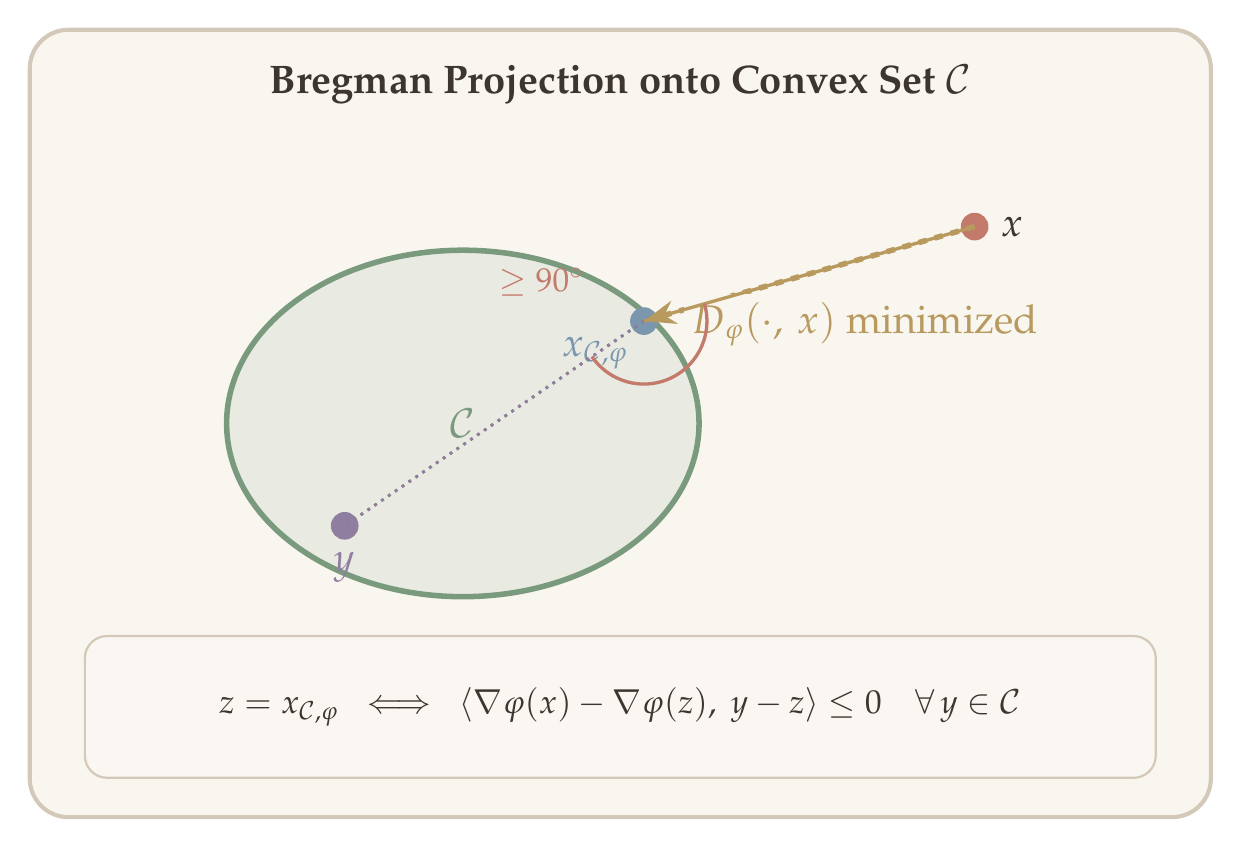
\begin{tikzpicture}[>={Stealth[length=4mm, width=3mm]}]

% Background
\fill[cream, rounded corners=14pt] (-1,-0.5) rectangle (14,9.5);
\draw[border, line width=1.5pt, rounded corners=14pt] (-1,-0.5) rectangle (14,9.5);

% Title
\node[text=dkbrown, font=\Large\bfseries] at (6.5,8.8)
  {Bregman Projection onto Convex Set $\mathcal{C}$};

% Convex set C (ellipse)
\coordinate (C) at (4.5,4.5);
\fill[sage, opacity=0.12] (C) ellipse (3.0 and 2.2);
\draw[sage, line width=2pt] (C) ellipse (3.0 and 2.2);
\node[text=sage, font=\Large\bfseries] at (4.5,4.5) {$\mathcal{C}$};

% Point x (outside the set)
\coordinate (xpt) at (11.0,7.0);
\fill[terracotta] (xpt) circle (5pt);
\node[text=dkbrown, font=\Large\bfseries, right=6pt] at (xpt) {$x$};

% Bregman projection x_{C,phi}
\coordinate (xc) at (6.8,5.8);
\fill[stblue] (xc) circle (5pt);
\node[text=stblue, font=\Large\bfseries, below left=3pt] at (xc) {$x_{\mathcal{C},\varphi}$};

% Point y (inside C)
\coordinate (ypt) at (3.0,3.2);
\fill[lavender] (ypt) circle (5pt);
\node[text=lavender, font=\Large\bfseries, below=6pt] at (ypt) {$y$};

% Arrow from x to x_{C,phi}
\draw[rwgold, line width=2pt, dashed, ->] (xpt) -- (xc);
\node[text=rwgold, font=\Large, fill=cream, inner sep=3pt] at ($(xpt)!0.45!(xc) + (0.5,-0.7)$)
  {$D_\varphi(\cdot,\, x)$ minimized};

% Characterization: angle condition at x_{C,phi}
% Draw lines from x_{C,phi} to y and from x_{C,phi} toward nabla phi direction
\draw[wmgray, line width=1pt, dotted] (xc) -- (ypt);

% Right angle indicator at x_{C,phi}
\coordinate (mid) at ($(xc)!0.35!(xpt)$);
\coordinate (mid2) at ($(xc)!0.35!(ypt)$);

% Annotation for the characterization
\fill[cream!90!white, rounded corners=8pt] (-0.3,0.0) rectangle (13.3,1.8);
\draw[border, line width=0.8pt, rounded corners=8pt] (-0.3,0.0) rectangle (13.3,1.8);
\node[text=dkbrown, font=\large, align=center] at (6.5,0.9)
  {$z = x_{\mathcal{C},\varphi} \;\iff\;
   \langle \nabla\varphi(x) - \nabla\varphi(z),\; y - z \rangle \leq 0
   \quad \forall\, y \in \mathcal{C}$};

% Obtuse angle visualization
\draw[rwgold, line width=1.2pt] (xc) -- ++($(xpt)-(xc)$) coordinate (dir1);
\draw[lavender, line width=1pt, dotted] (xc) -- (ypt);

% Small angle arc
\draw[terracotta, line width=1.2pt]
  let \p1 = ($(xpt)-(xc)$),
      \p2 = ($(ypt)-(xc)$),
      \n1 = {atan2(\y1,\x1)},
      \n2 = {atan2(\y2,\x2)}
  in (xc) ++(\n1:0.8) arc (\n1:\n2:0.8);
\node[text=terracotta, font=\large] at ($(xc) + (-1.3,0.5)$) {$\geq 90^\circ$};

\end{tikzpicture}
\end{document}
